\Chapter{ETUDE DE LA RESISTANCE D'UNE ROUE CYR}\label{sec:Theme3}

\section{Masse minimale}

Réduire la masse de la roue Cyr revient à enlever de la matière. Il existe donc une masse minimale en dessous de laquelle la roue ne pourra pas résister aux contraintes induites par le poids de l'utilisateur.

\begin{itemize}
    \item On commence par calculer les contraintes lorsque la roue est comprimée par une force $F$: La contrainte dans l'arrête extérieure s'exprime $\sigma_i=k_i\sigma$ \cite{roark},
    où sigma est la contrainte calculée pour une poutre droite: $\sigma=\frac{Mr_2}{I_z}$, avec $I_z=\frac{\pi}{2}(r_2^4-r_1^4)$ et $M=\frac{\pi}{4}FR$.
    D'après les formules du livre de Roark, $k_i$ s'exprime $k_i=\frac{1}{4\beta}\frac{1-\beta}{\frac{R_c}{r_2}-1}[1+(\frac{r_1}{r_2})^2]$ avec $\beta=\frac{1}{2}[\frac{2R_c}{r_2}-\sqrt{(\frac{R_c}{r_2})^2-1}-\sqrt{(\frac{R_c}{r_2})^2-(\frac{r_1}{r_2})^2}]$ 
    \item Il ne reste plus qu'à déterminer le rayon de courbure de la roue comprimée, comme illustré sur la figure \ref{fig:ellr}: $R_c=\frac{a_r^2}{b_r}$, $a_r$ et $b_r$ étant respectivement les demi grand axe et demi petit axe de l'ellipse que devient la roue lorsqu'elle est comprimée.\\
    
    \begin{figure}[htb]
    \centering
    %% Creator: Inkscape inkscape 0.92.2, www.inkscape.org
%% PDF/EPS/PS + LaTeX output extension by Johan Engelen, 2010
%% Accompanies image file 'ellipse.eps' (pdf, eps, ps)
%%
%% To include the image in your LaTeX document, write
%%   \input{<filename>.pdf_tex}
%%  instead of
%%   \includegraphics{<filename>.pdf}
%% To scale the image, write
%%   \def\svgwidth{<desired width>}
%%   \input{<filename>.pdf_tex}
%%  instead of
%%   \includegraphics[width=<desired width>]{<filename>.pdf}
%%
%% Images with a different path to the parent latex file can
%% be accessed with the `import' package (which may need to be
%% installed) using
%%   \usepackage{import}
%% in the preamble, and then including the image with
%%   \import{<path to file>}{<filename>.pdf_tex}
%% Alternatively, one can specify
%%   \graphicspath{{<path to file>/}}
%% 
%% For more information, please see info/svg-inkscape on CTAN:
%%   http://tug.ctan.org/tex-archive/info/svg-inkscape
%%
\begingroup%
  \makeatletter%
  \providecommand\color[2][]{%
    \errmessage{(Inkscape) Color is used for the text in Inkscape, but the package 'color.sty' is not loaded}%
    \renewcommand\color[2][]{}%
  }%
  \providecommand\transparent[1]{%
    \errmessage{(Inkscape) Transparency is used (non-zero) for the text in Inkscape, but the package 'transparent.sty' is not loaded}%
    \renewcommand\transparent[1]{}%
  }%
  \providecommand\rotatebox[2]{#2}%
  \ifx\svgwidth\undefined%
    \setlength{\unitlength}{318.40595442bp}%
    \ifx\svgscale\undefined%
      \relax%
    \else%
      \setlength{\unitlength}{\unitlength * \real{\svgscale}}%
    \fi%
  \else%
    \setlength{\unitlength}{\svgwidth}%
  \fi%
  \global\let\svgwidth\undefined%
  \global\let\svgscale\undefined%
  \makeatother%
  \begin{picture}(1,0.51062056)%
    \put(0,0){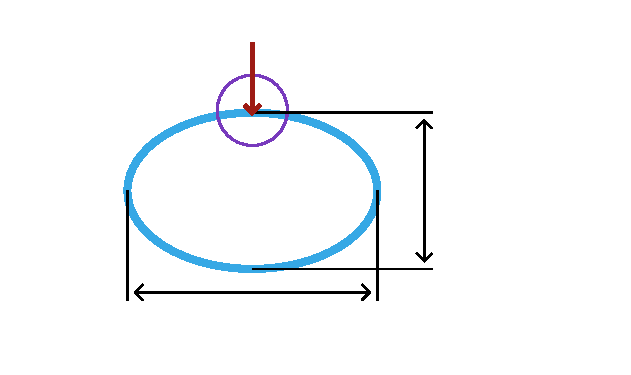
\includegraphics[width=\unitlength]{images_contraintes/ellipse.eps}}%
    \put(0.69807629,0.26119896){\color[rgb]{0,0,0}\makebox(0,0)[lb]{\smash{$2a_r$}}}%
    \put(0.380830868,0.06042804){\color[rgb]{0,0,0}\makebox(0,0)[lb]{\smash{$2b_r$}}}%
    \put(0.34402215,0.52558617){\color[rgb]{0.61568627,0.10588235,0.07843137}\makebox(0,0)[lb]{\smash{$F$}}}%
    \put(0.45664975,0.45341089){\color[rgb]{0.47058824,0.22745098,0.74117647}\makebox(0,0)[lb]{\smash{zone où les contraintes sont maximales}}}%
    \put(0.82651502,0.40252801){\color[rgb]{0,0,0}\makebox(0,0)[lb]{\smash{}}}%
  \end{picture}%
\endgroup%

    \caption{Représentation schématique d'un tore plié par une force de compression F. Il devient une ellipse de demi grand axe $a_r$ et de demi petit axe $b_r$. La zone où les contraintes sont maximales correspond à l'endroit où la force est appliquée.}
    \label{fig:ellr}
    \end{figure}
    
\begin{itemize}
    \item Pour calculer $a_r$ et $b_r$, on utilise les formules du livre de Roark qui donnent les variations de diamètre horizontal $\Delta D_h$ et vertical $\Delta D_v$ d'une anneau comprimé selon son diamètre avec une force $F$, et on aura ainsi $a_r=R+\frac{\Delta D_h}{2}$ et $b_r=R+\frac{\Delta D_v}{2}$.
    \item D'après les formules de Roark, $\Delta D_h=\frac{FR^3}{EI}(\frac{1}{2}(1+\frac{I}{AR^2}+\frac{2EI}{GAR^2})-1+\frac{2}{/pi}(1-\frac{I}{AR^2})^2)$ et $\Delta D_v=-\frac{FR^3}{EI}(\frac{\pi}{4}(1-\frac{I}{AR^2}+\frac{2EI}{GAR^2})-\frac{2}{/pi}(1-\frac{I}{AR^2})^2)$, où $A$ est l'aire de section, $E$, le module de Young, $G$, le module de cisaillement, $R$, le rayon médian de la roue, et $I$ le moment de section quadratique selon l'axe principal perpendiculaire au plan de la roue.
    \item En implémentant numériquement les équations ci-dessus, on est capable de calculer les contraintes maximales auxquelles sera soumise la roue pour une force de compression $F$ donnée. Pour $F=900N$, en fixant $r_2$ et en faisant varier $r_1$ de $0$ à $r_2$, on est capable de tracer les contraintes maximales, en fonction de la masse de la roue, $m_r=2\pi\rho A R$. Comme l'illustre la figure-\ref{fig:mmin1} ci-dessous, il est alors possible de déterminer la masse à partir de laquelle les contraintes passent sous le seuil de $63 MPa$, et donc à partir de laquelle il y a rupture.
    
\end{itemize}


\begin{figure}[htb]
\centering
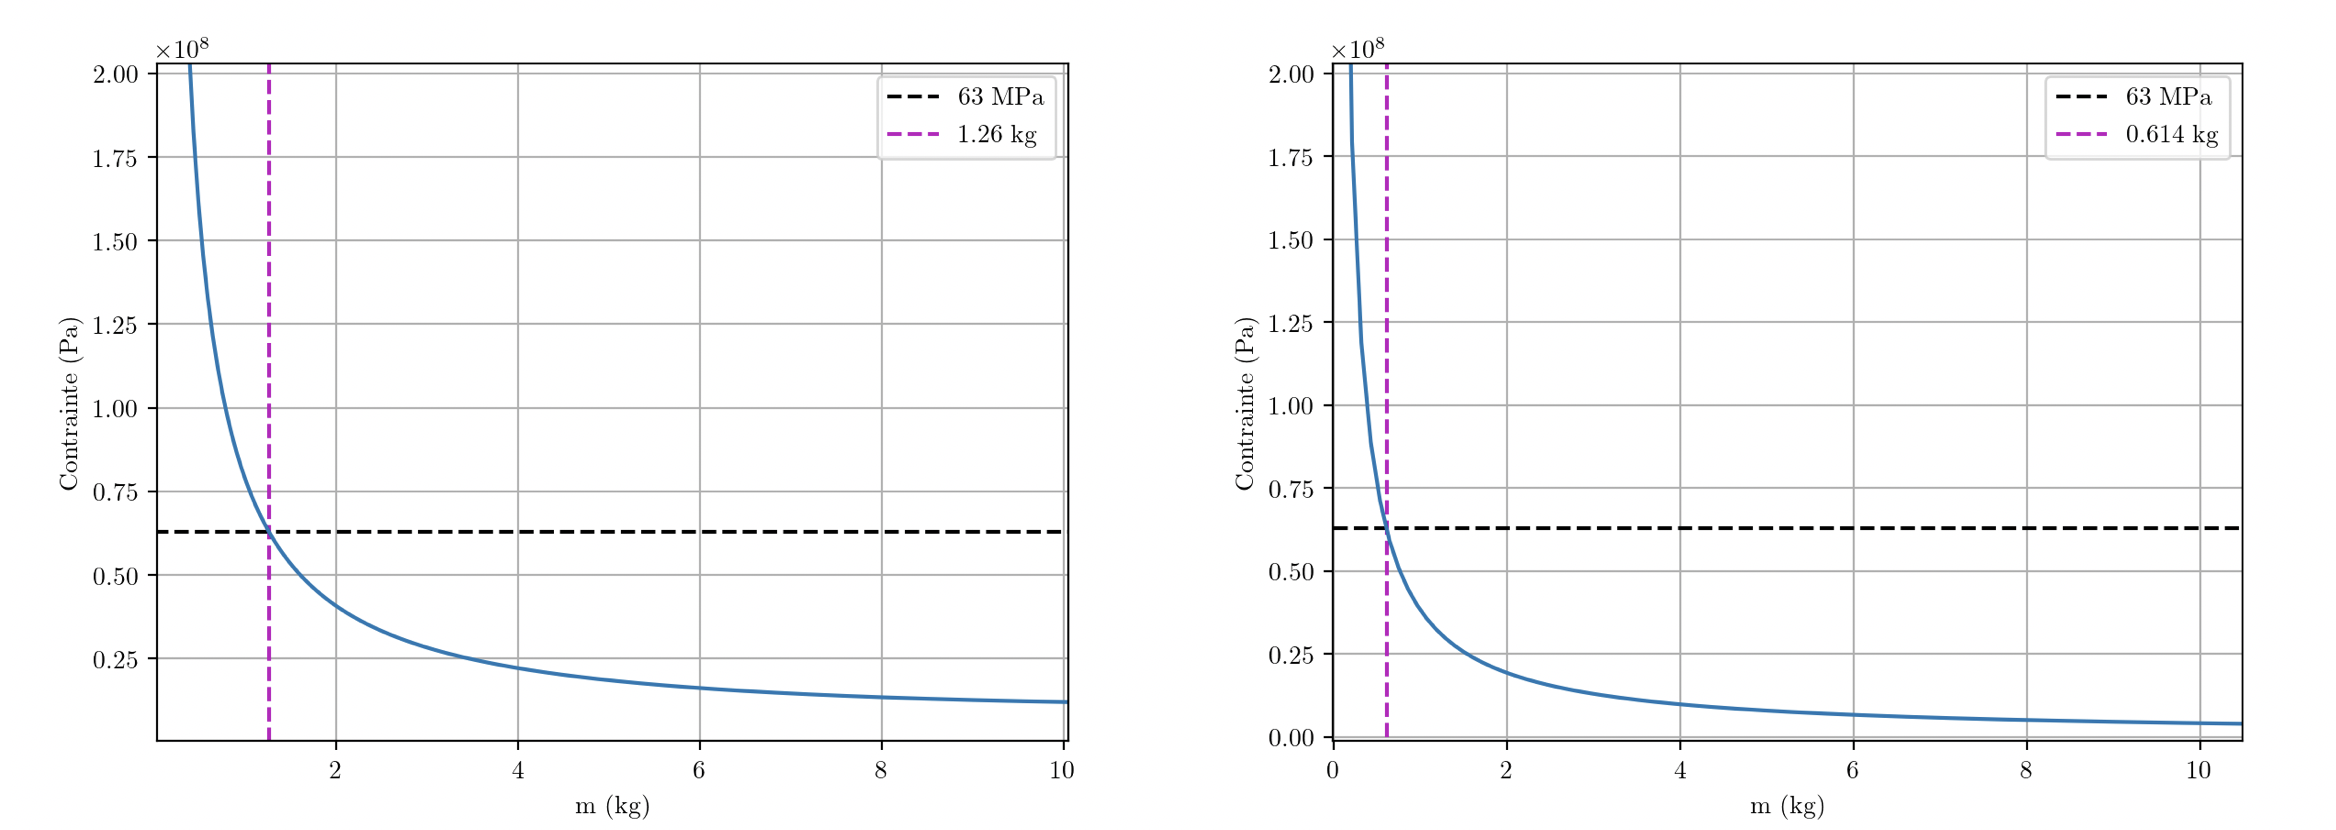
\includegraphics[width=7in]{images_2ddl/mmin1.png}
\caption{Contraintes maximales dans la roue en fonction de sa masse, la courbe de gauche correspond à un rayon de section externe $r_2=2.5 cm$ et un rayon de section interne $r_1$ variant de $0.0$ à $2.49 cm$. La courbe de droite correspond à à $r_2=5.0 cm$ et $r_1$ variant de $0.0$ à $4.99 cm$}
\label{fig:mmin1}
\end{figure}


\begin{itemize}
    \item On peut donc implémenter ce procédé numériquement pour déterminer cette valeur minimale de la masse pour en fonction de $r_2$. Le resultat de l'implémentation est présenté à la figure-\ref{fig:mmin2} ci-dessous. 
\end{itemize}


\begin{figure}[htb]
\centering
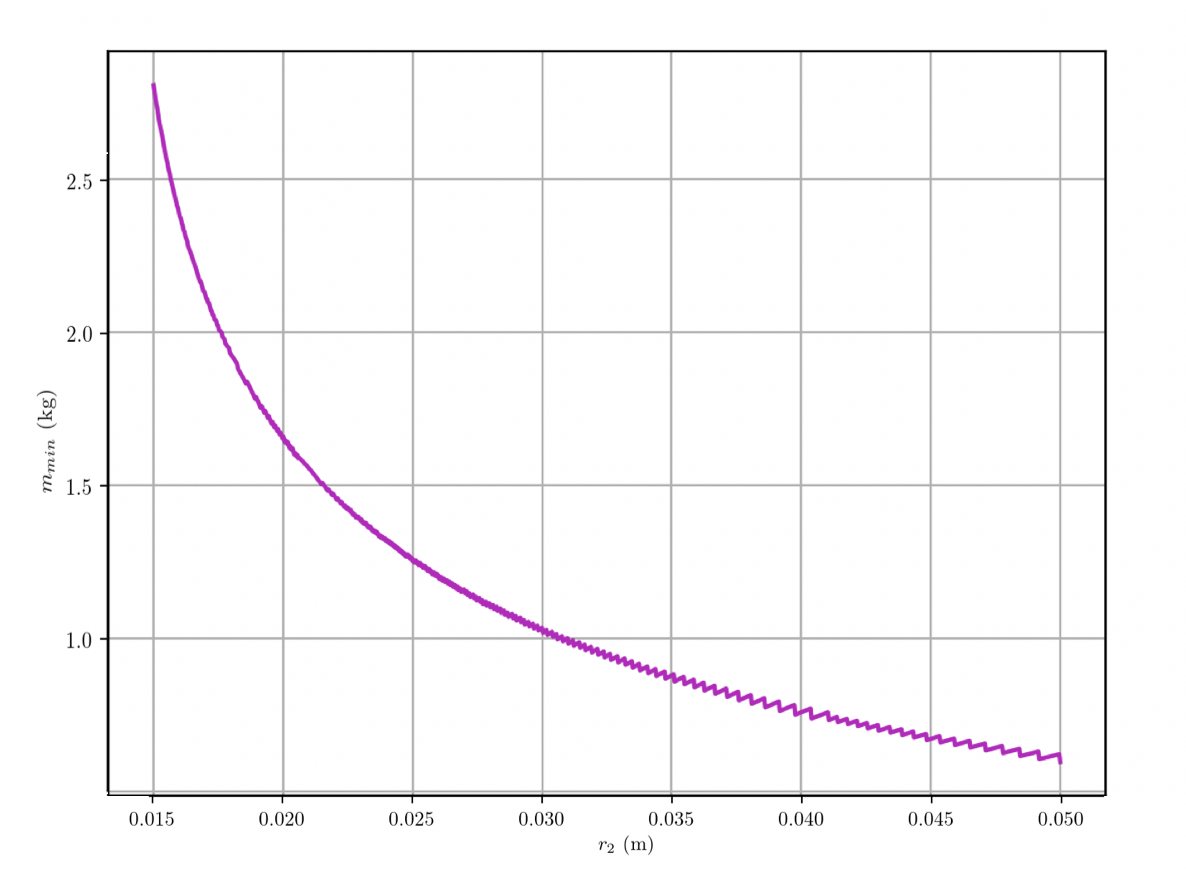
\includegraphics[width=4in]{images_2ddl/mmin2.png}
\caption{Masse minimale de la roue en fonction de $r_2$}
\label{fig:mmin2}
\end{figure}


\item Pour ce qui suit, $r_2$ sera fixé à $1.75 cm$, la masse minimale sera donc $2.0 kg$
\end{itemize}
